\documentclass[border=0pt]{standalone}
\usepackage{pgfplots}
\pgfplotsset{width=\linewidth,compat=1.8}
\usepackage{amsmath}
\usepackage{pgfplotstable}
\usepgfplotslibrary{fillbetween}
\providecommand{\datapath}{.}


\pgfplotsset{every tick label/.append style={font=\boldmath\Huge}}
\tikzstyle{every node}=[font=\bfseries\Huge]

\begin{document}
\pgfplotstableread[col sep=comma,]{\datapath/dcfr9_2.csv}\dcfrb
\pgfplotstableread[col sep=comma,]{\datapath/dcfr16_2.csv}\dcfra
\pgfplotstableread[col sep=comma,]{\datapath/cams_2.csv}\cams
 \LARGE
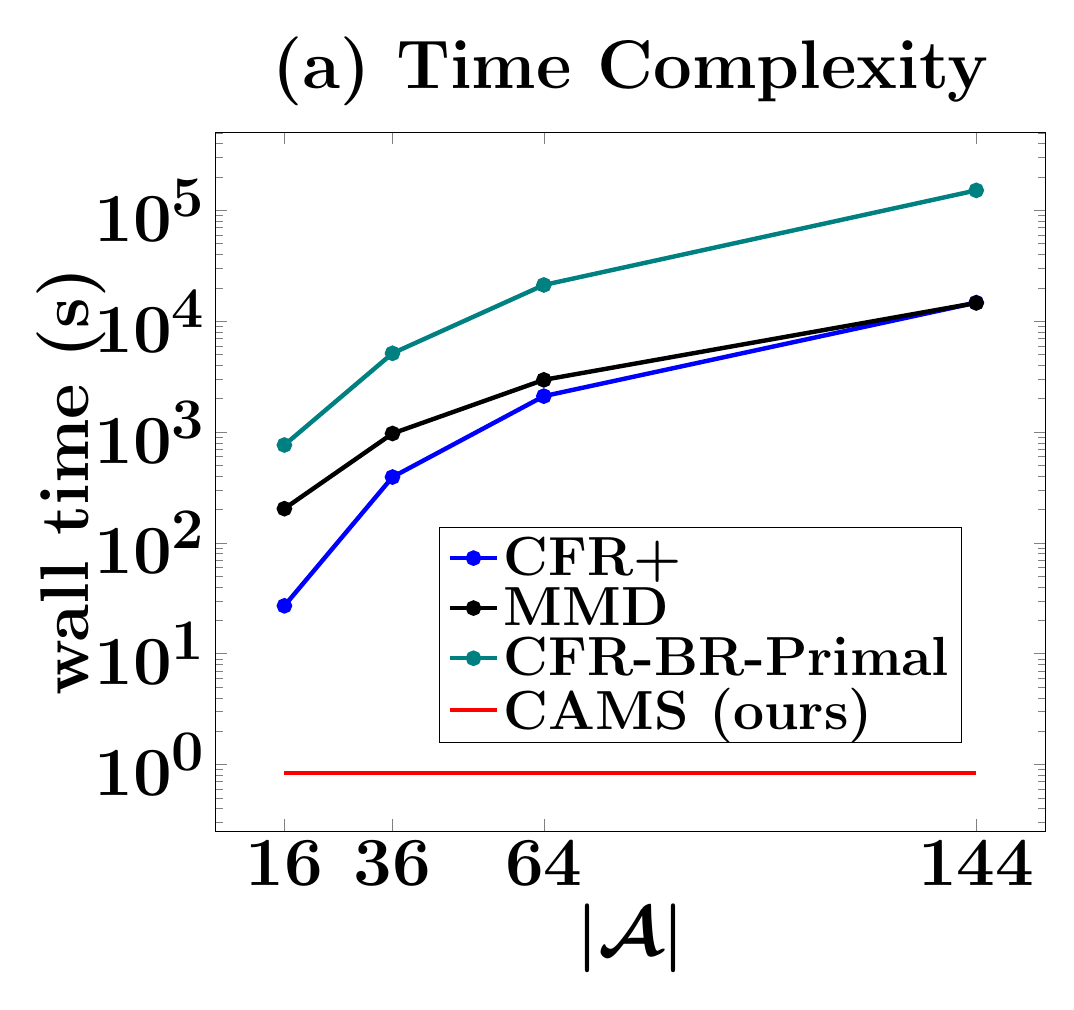
\begin{tikzpicture}[scale=1]
\begin{axis}[title={(a) Time Complexity},
    legend style={nodes={scale=0.8}, style={at={(0.9, 0.435)}}, fill=none},
    legend cell align={left},
    legend entries={CFR+, MMD, CFR-BR-Primal, CAMS (ours)},
    xlabel={$\boldsymbol{|\mathcal{A}|}$},
    ylabel={\textbf{wall time (s)}},
    xtick={16, 36, 64, 144},
    ymode=log,
    % xmode=log,
    ylabel shift=-11pt,
]
% cfr+
\addplot [mark=*, mark size=2pt, ultra thick, blue] coordinates {
(16, 27.05)
(36, 392.77)
(64, 2108.81)
(144, 14707.94)
};
%mmd
\addplot [ultra thick, black, mark=*, mark size=2pt] coordinates {
(16, 203.58)
(36, 970.45)
(64, 2958.36)
(144, 14629.44)
};
%cfr-br-primal
\addplot [ultra thick, teal, mark=*, mark size=2pt] coordinates {
(16, 764)
(36, 5136)
(64, 21238)
(144, 151596)
};
% cams
\addplot [ultra thick, red] coordinates {
(16, 0.842)
(36, 0.842)
(64, 0.842)
(144, 0.842)
};

\end{axis}
\end{tikzpicture}%
% iterations count
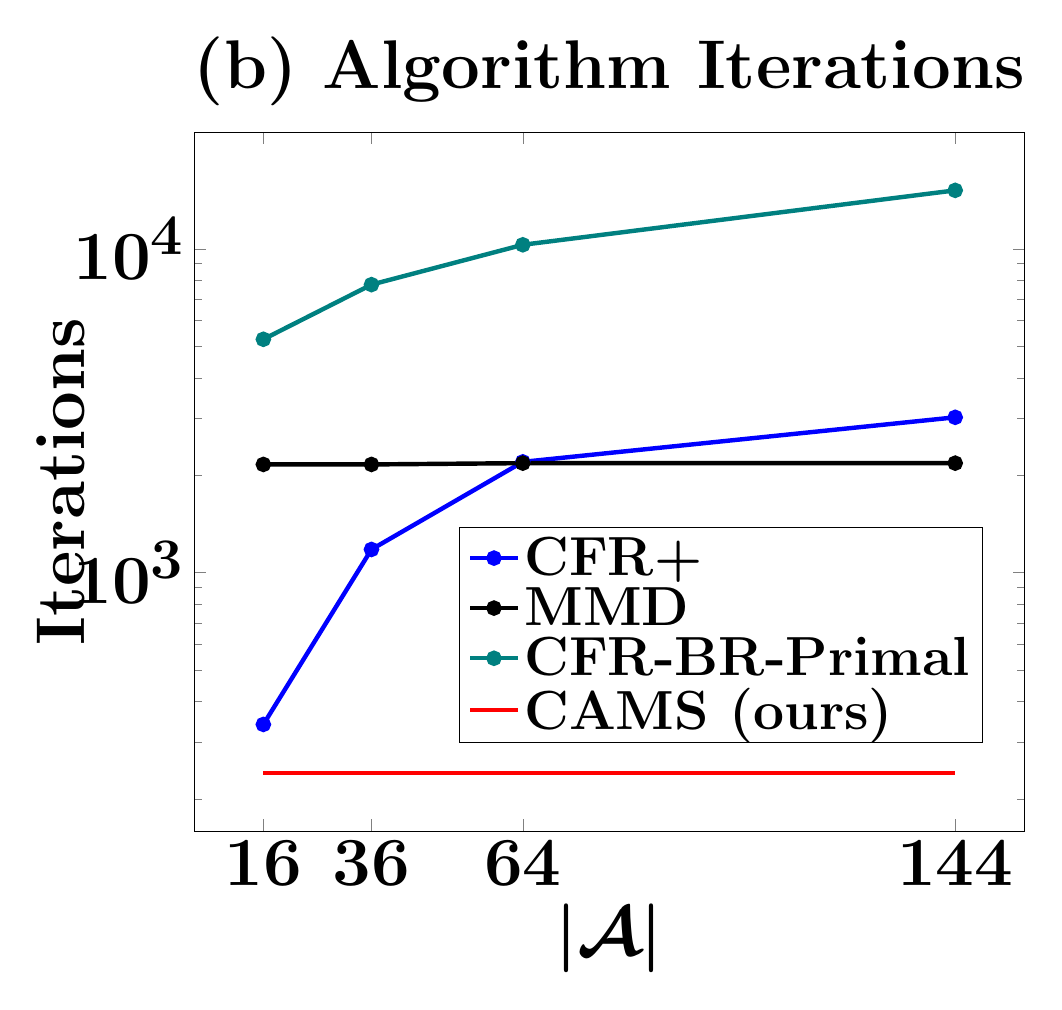
\begin{tikzpicture}[scale=1]
\begin{axis}[title={(b) Algorithm Iterations},
    legend style={nodes={scale=0.8}, style={at={(0.95, 0.435)}}, fill=none},
    legend cell align={left},
    legend entries={CFR+, MMD, CFR-BR-Primal, CAMS (ours)},
    xlabel={$\boldsymbol{|\mathcal{A}|}$},
    ylabel={\textbf{Iterations}},
    xtick={16, 36, 64, 144},
    ymode=log,
    ylabel shift=-11pt,
    % ytick distance=10^.4,
    % log ticks with fixed point,
    % ymin=1e1,
    % ytick={150, 1000, 7000},
    % ytick = {1, 10^1, 10^2, 10^3},
]
% cfr+
\addplot [mark=*, mark size=2pt, ultra thick, blue] coordinates {
(16, 340)
(36, 1180)
(64, 2200)
(144, 3020)
};
%mmd
\addplot [ultra thick, black, mark=*, mark size=2pt] coordinates {
(16, 2160)
(36, 2160)
(64, 2180)
(144, 2180)
};
% cfr-br-primal
\addplot [mark=*, mark size=2pt, ultra thick, teal] coordinates {
(16, 5260)
(36, 7760)
(64, 10300)
(144, 15169)
};
% cams
\addplot [ultra thick, red] coordinates {
(16, 241)
(36, 241)
(64, 241)
(144, 241)
};

\end{axis}
\end{tikzpicture}%
% distance to gt
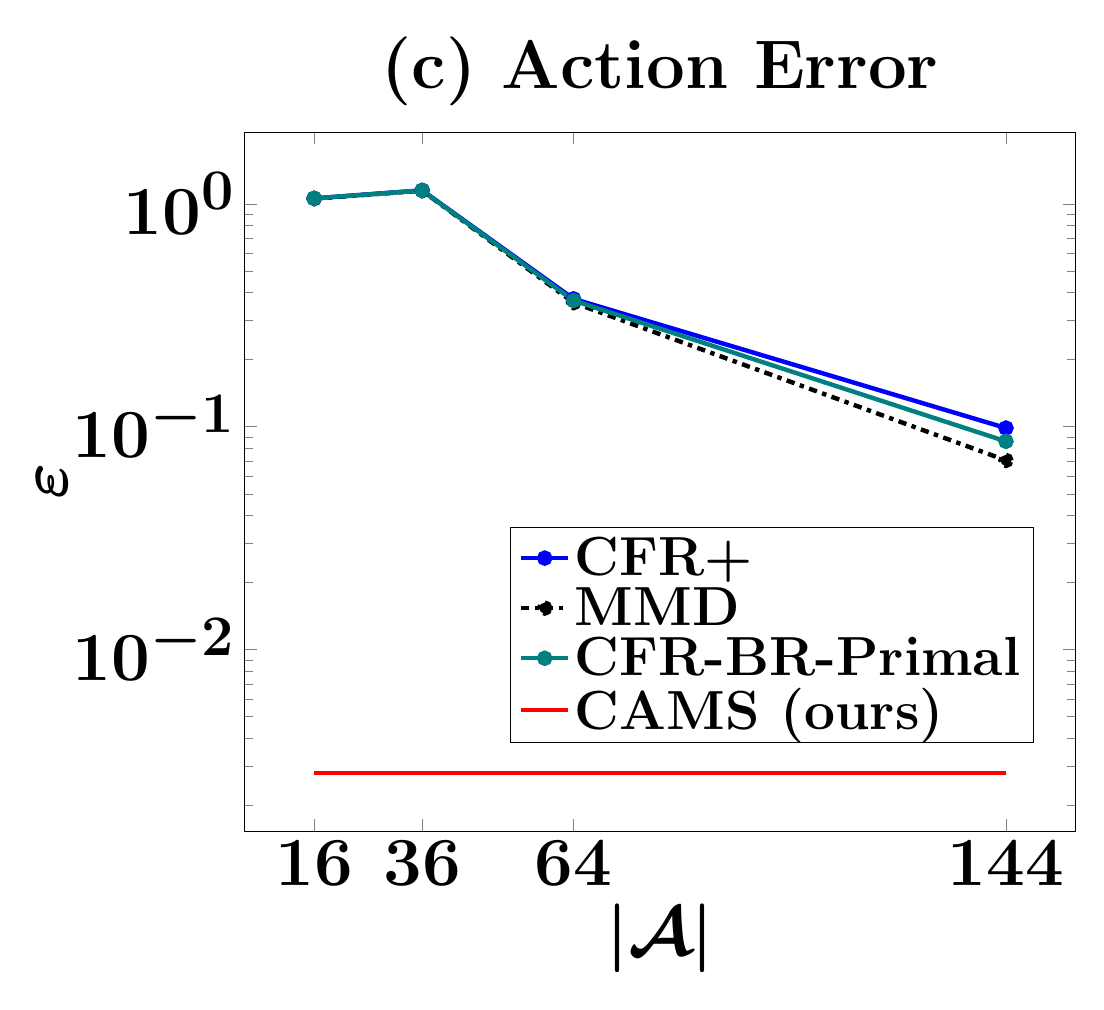
\begin{tikzpicture}[scale=1]
\begin{axis}[title={(c) Action Error},
    legend style={nodes={scale=0.8}, style={at={(0.95, 0.435)}}, fill=none},
    legend cell align={left},
    legend entries={CFR+, MMD, CFR-BR-Primal, CAMS (ours)},
    xlabel={$\boldsymbol{|\mathcal{A}|}$},
    ylabel={$\boldsymbol{\varepsilon}$},
    xtick={16, 36, 64, 144},
    ymode=log,
    ylabel shift=-5pt,
]
% cfr+
\addplot [mark=*, mark size=2pt, ultra thick, blue] coordinates {
(16, 1.0588427800973248)
(36, 1.1494801917079402)
(64, 0.37464195668540257)
(144, 0.09866226893665803)
};
% mmd
% mmd
% [0.5552314866840433,
%  0.5209049957759864,
%  0.5586684894950396,
%  0.6097465051451072]
\addplot[ultra thick, black, mark=*, mark size=2pt, dashdotted] coordinates {
(16, 1.0552507678615948)
(36, 1.146136600348143)
(64, 0.36045590244936615)
(144, 0.07065840307433174)
};
% cfr-br-primal
% 0.6496365514625374,
%  0.2945435474633056,
%  0.1709301707831794,
%  0.03248224069686917
\addplot[ultra thick, mark=*, mark size=2pt, teal] coordinates{
% (16, 0.524)
% (36, 0.568)
% (64, 0.157)
% (144, 0.031)
(16, 1.0581758567678188)
(36, 1.1486716970232314)
(64, 0.3682825954941562)
(144, 0.08599092519673776)
};
% cams
\addplot [ultra thick, red] coordinates {
(16, 0.0028)
(36, 0.0028)
(64, 0.0028)
(144, 0.0028)
};
\end{axis}
\end{tikzpicture}%
\begin{tikzpicture}[scale=1.03]
    \begin{axis}[title={(d) Action Error}, every axis title/.style={above, at={(0.5, 0.986)}},
    legend style={nodes={scale=0.8}, style={at={(0.9, 0.38)}}, fill=none},
    legend cell align={left},
    legend entries={DeepCFR $\boldsymbol{(|\mathcal{A}|=16)}$, DeepCFR $\boldsymbol{(|\mathcal{A}|=9)}$, CAMS (ours)},
    xlabel={$\boldsymbol{t}$},
    ylabel={$\boldsymbol{\bar{\varepsilon}_t}$},
    xtick={0, 0.25, 0.5, 0.75},
    % ytick={0, 5, 10, 15},
    % ymode=log,
    xmax=0.8,
    ylabel shift=-5pt,
]   
% A =16
\addplot [mark=*, mark size=2pt, ultra thick, blue] table[x=x,y=y] {\dcfra};
% A =9
\addplot [mark=*, mark size=2pt, ultra thick, teal] table[x=x,y=y] {\dcfrb};
% cams
\addplot [mark=*, mark size=2pt, ultra thick, red] table[x=x,y=y] {\cams};
% fill betweens
% cfr_9
\addplot [name path=upper,draw=none] table[x=x,y expr=\thisrow{y}+\thisrow{err}] {\dcfrb};
\addplot [name path=lower,draw=none] table[x=x,y expr=\thisrow{y}-\thisrow{err}] {\dcfrb};
\addplot [fill=teal!40, fill opacity=0.4] fill between[of=upper and lower];
% cfr_16
\addplot [name path=upper_2,draw=none] table[x=x,y expr=\thisrow{y}+\thisrow{err}] {\dcfra};
\addplot [name path=lower_2,draw=none] table[x=x,y expr=\thisrow{y}-\thisrow{err}] {\dcfra};
\addplot [fill=blue!40, fill opacity=0.4] fill between[of=upper_2 and lower_2];
% cams
\addplot [name path=upper_3,draw=none] table[x=x,y expr=\thisrow{y}+\thisrow{err}] {\cams};
\addplot [name path=lower_3,draw=none] table[x=x,y expr=\thisrow{y}-\thisrow{err}] {\cams};
\addplot [fill=red!10] fill between[of=upper_3 and lower_3];
    \end{axis}
\end{tikzpicture}
\end{document}